\documentclass[final,20pt]{beamer}
% ====================
% Packages
% ====================

\usepackage[T1]{fontenc}
\usepackage{lmodern}
% change the orientation to landscape if needed
\usepackage[orientation=portrait,size=a0paper,scale=1.1]{beamerposter}
\usetheme{gemini}
\usecolortheme{uhb}
\usepackage{graphicx}
\usepackage[nameinlink]{cleveref}
\usepackage[protrusion=true,expansion]{microtype}
\usepackage[inkscapeformat=png]{svg}
\usepackage{booktabs}
\usepackage{tikz}
\usetikzlibrary{shapes.symbols}
\usetikzlibrary{shapes.arrows}
\usepackage{pgfplots}
\pgfplotsset{compat=1.18}
\usepackage{anyfontsize}
\usepackage[style=alphabetic,backend=biber]{biblatex}
\addbibresource{poster.bib}
\usepackage{wrapfig}
\usepackage{subcaption}
\usepackage{setspace}
% ====================
% Lengths
% ====================
% 1.5 Zeilenabstand
%\onehalfspacing%

% If you have N columns, choose \sepwidth and \colwidth such that
% (N+1)*\sepwidth + N*\colwidth = \paperwidth
\newlength{\blocksep}
\newlength{\sepwidth}
\newlength{\colwidth}
\setlength{\blocksep}{0.05\pageheight}
\setlength{\sepwidth}{0.025\paperwidth}
\setlength{\colwidth}{0.3\paperwidth}
% Uppercase Figure references 
\crefname{figure}{Figure}{Figures}
\newcommand{\separatorcolumn}{\begin{column}{\sepwidth}\end{column}}

% ====================
% Title
% ====================

\title{Land Use Change and Climate Change Impact on \newline Urban Heat Islands Development}

\author{Linus Andrae\inst{1}}

\institute[shortinst]{\inst{1} Institute for Environmental Physics, University of Bremen}

% ====================
% Footer (optional)
% ====================

\footercontent{%

  \begin{columns}[t]
    \begin{column}{\colwidth+5cm}
      \begin{wrapfigure}{l}{6cm}     
        \centering
        \vspace{-2cm}
        
\includegraphics[width=5cm]{figures/qr-code}
      \end{wrapfigure}
      \href{https://github.com/paradx/PresTPoster/blob/main/poster.pdf?raw=true}{The online version of this Poster: \\%
      https://github.com/paradx/PresTPoster/blob/main/poster.pdf?raw=true} \vspace{1cm}
    \end{column}
    \begin{column}{\colwidth}
      \centering
      \vfill
        Summery of Master Thesis Results \\ Space Science and Technology M.Sc. \\ University Bremen \hfill
    \end{column}
    \separatorcolumn%
    \begin{column}{\colwidth}
      \vfill
      \href{mailto:landrae@uni-bremen.de}{contact: landrae@uni-bremen.de}\\
    \end{column}
  \end{columns}
  }
% (can be left out to remove footer)

% ====================
% Logo (optional)
% ====================
% use this to include logos on the left and/or right side of the header:
\logoright{
\includegraphics[height=5cm]{logos/logoIUP.png}}
\logoleft{\includegraphics[height=5cm]{logos/logoDC.png}}

% ===================
% Configuration of blocks
% ==================

\addtobeamertemplate{block begin}
  {}
  {\vspace{1ex plus 0.5ex minus 0.5ex} % Pads top of block
     % separates paragraphs in a block
   \setlength{\parskip}{24pt plus 1pt minus 1pt}%
   \begin{adjustwidth}{2cm}{2cm}
  }
\addtobeamertemplate{block end}
  {\end{adjustwidth}%
   \vspace{2ex plus 0.5ex minus 0.5ex}}% Pads bottom of block
  {\vspace{\blocksep}} % Seperates blocks from each other

\addtobeamertemplate{block alerted begin}
  {}
  {\vspace{1ex plus 0.5ex minus 0.5ex} % Pads top of block
     % separates paragraphs in a block
   \setlength{\parskip}{24pt plus 1pt minus 1pt}%
   \begin{adjustwidth}{2cm}{2cm}
  }
\addtobeamertemplate{block alerted end}
  {\end{adjustwidth}%
   \vspace{2ex plus 0.5ex minus 0.5ex}}% Pads bottom of block
  {\vspace{\blocksep}} % Seperates blocks from each other

\addtobeamertemplate{block example begin}
  {}
  {\vspace{1ex plus 0.5ex minus 0.5ex} % Pads top of block
     % separates paragraphs in a block
   \setlength{\parskip}{24pt plus 1pt minus 1pt}%
   \begin{adjustwidth}{2cm}{2cm}
  }
\addtobeamertemplate{block example end}
  {\end{adjustwidth}%
   \vspace{2ex plus 0.5ex minus 0.5ex}}% Pads bottom of block
  {\vspace{\blocksep}} % Seperates blocks from each other

% ====================
% Body
% ====================

\begin{document}

\begin{frame}[t]
\tikz[remember picture, overlay] \node[opacity=0.3, yshift=-1cm] at (current page.center){\includegraphics[width=\textwidth,height=0.99\textheight]{figures/overlay}};
\begin{columns}[t]
\separatorcolumn%

\begin{column}{\colwidth}

  \begin{alertblock}{Introduction}
    Urban Heat Islands are a phenomenon, where the temperature within a city is significantly higher compared to the temperature of the surrounding rural area. \\
    \begin{itemize}\setlength{\itemsep}{0.5em}
      \item \textbf{Goal:} Detection and Analysis of UHIs using Landsat 8 \& 9 Satellite Data:
      \item \textbf{Why} Find influencing factors on size and impact of urbanisation and climate change of UHIs
      \item \textbf{Output} Find factors that influence UHI severity and size. Determine what indices are useful for judging impact of UHI on human health
    \end{itemize}
  \end{alertblock}

  \begin{exampleblock}{Urban Heat Islands}
    \begin{itemize}\setlength{\itemsep}{0.5em}
      \item \textbf{Urban Heat Islands} (UHIs) $\rightarrow$ Surface and air temperature within a city is higher than the average temperature of the surrounding area.
      \item \textbf{Consequences} $\rightarrow$ Major health impact, increased pollution, reduced well-being 
      \item \textbf{Measurement Technique} $\rightarrow$ Remote sensing data for Surface UHIs and local weather station measurements for Atmospheric UHIs
    \end{itemize}
  \end{exampleblock}


  \begin{block}{Processing Chain}
   The Image Processing Pipeline can be separated in these steps:
    \begin{enumerate}
      \setlength\itemsep{0.3em}
      \item \textbf{Preprocessing} Cutting the image area to the area of interested
      \item \textbf{Feature Engineering} A Gabor filter bank of rotated Gabor kernels is used to enrich pixels with information about surrounding pixel and larger structures.
      \item \textbf{Image Classification}  The pixels are classified using a k-means based classification. 
      \item \textbf{Urban Area Detection} Classes indicating urban areas are identified and the buffer zones are build up around the areas to calculate a reference temperature.
      \item \textbf{Peri-Urban Area Clean-up} Larger settlement structures are masked away in the surrounding areas
      \item \textbf{Detection of Urban Heat Islands} using thermal infrared images to detect UHIs within the Urban Area
      \item \textbf{Statistical Analysis of UHIs} Pixel within the UHI are evaluated using land surface type, NDVI and NDBI as well as LST values 
      \item \textbf{Timeline Creation} Repetition of the pipeline for different images of the same area over multiple years:
        \begin{itemize}
          \setlength\itemsep{0.5em}
          \item change in size of UHIs 
          \item statistical composition of UHIs 
        \end{itemize}
      \setlength\itemsep{0.5em}
      \item \textbf{Result} Correlating of UHI with climate and land use change 
    \end{enumerate}
  \end{block}

\end{column}

\separatorcolumn%

\begin{column}{\colwidth}
  \begin{block}{Feature Engineering}
  For adding information of surrounding larger scale structures to each pixels, for each image band the same bank of Gabor-filters was used. 
  \begin{itemize}
          \setlength\itemsep{0.5em}
    \item \textbf{Gabor filter}$\rightarrow$ convolution of a sinosoid and a gaussian.
    \item \textbf{parameter variation} $\sigma$ of gaussian, $\nu$, $\lambda$ and $\phi$ of sine
    \item \textbf{Output} Detection of patterns, structures and textures in different orientations and sizes
    \item \textbf{Additional information} one binary marker if pixel is part of larger structure
  \end{itemize}
  The result of the convolution of the filter in \cref{fig:filter} with an Landsat 8 image is shown in \cref{fig:feats}. \\ 
     \begin{figure}
       \begin{subfigure}{0.47\linewidth}
      \centering
      \includegraphics[width=0.9\linewidth]{figures/K5.png}
      \subcaption{Example filter bank of 90\textdegree\ rotated Gabor-kernel with $\sigma = 2$, $f = 0.15$\label{fig:filter}} 
    \end{subfigure}
    \begin{subfigure}{0.47\linewidth}
      \centering
      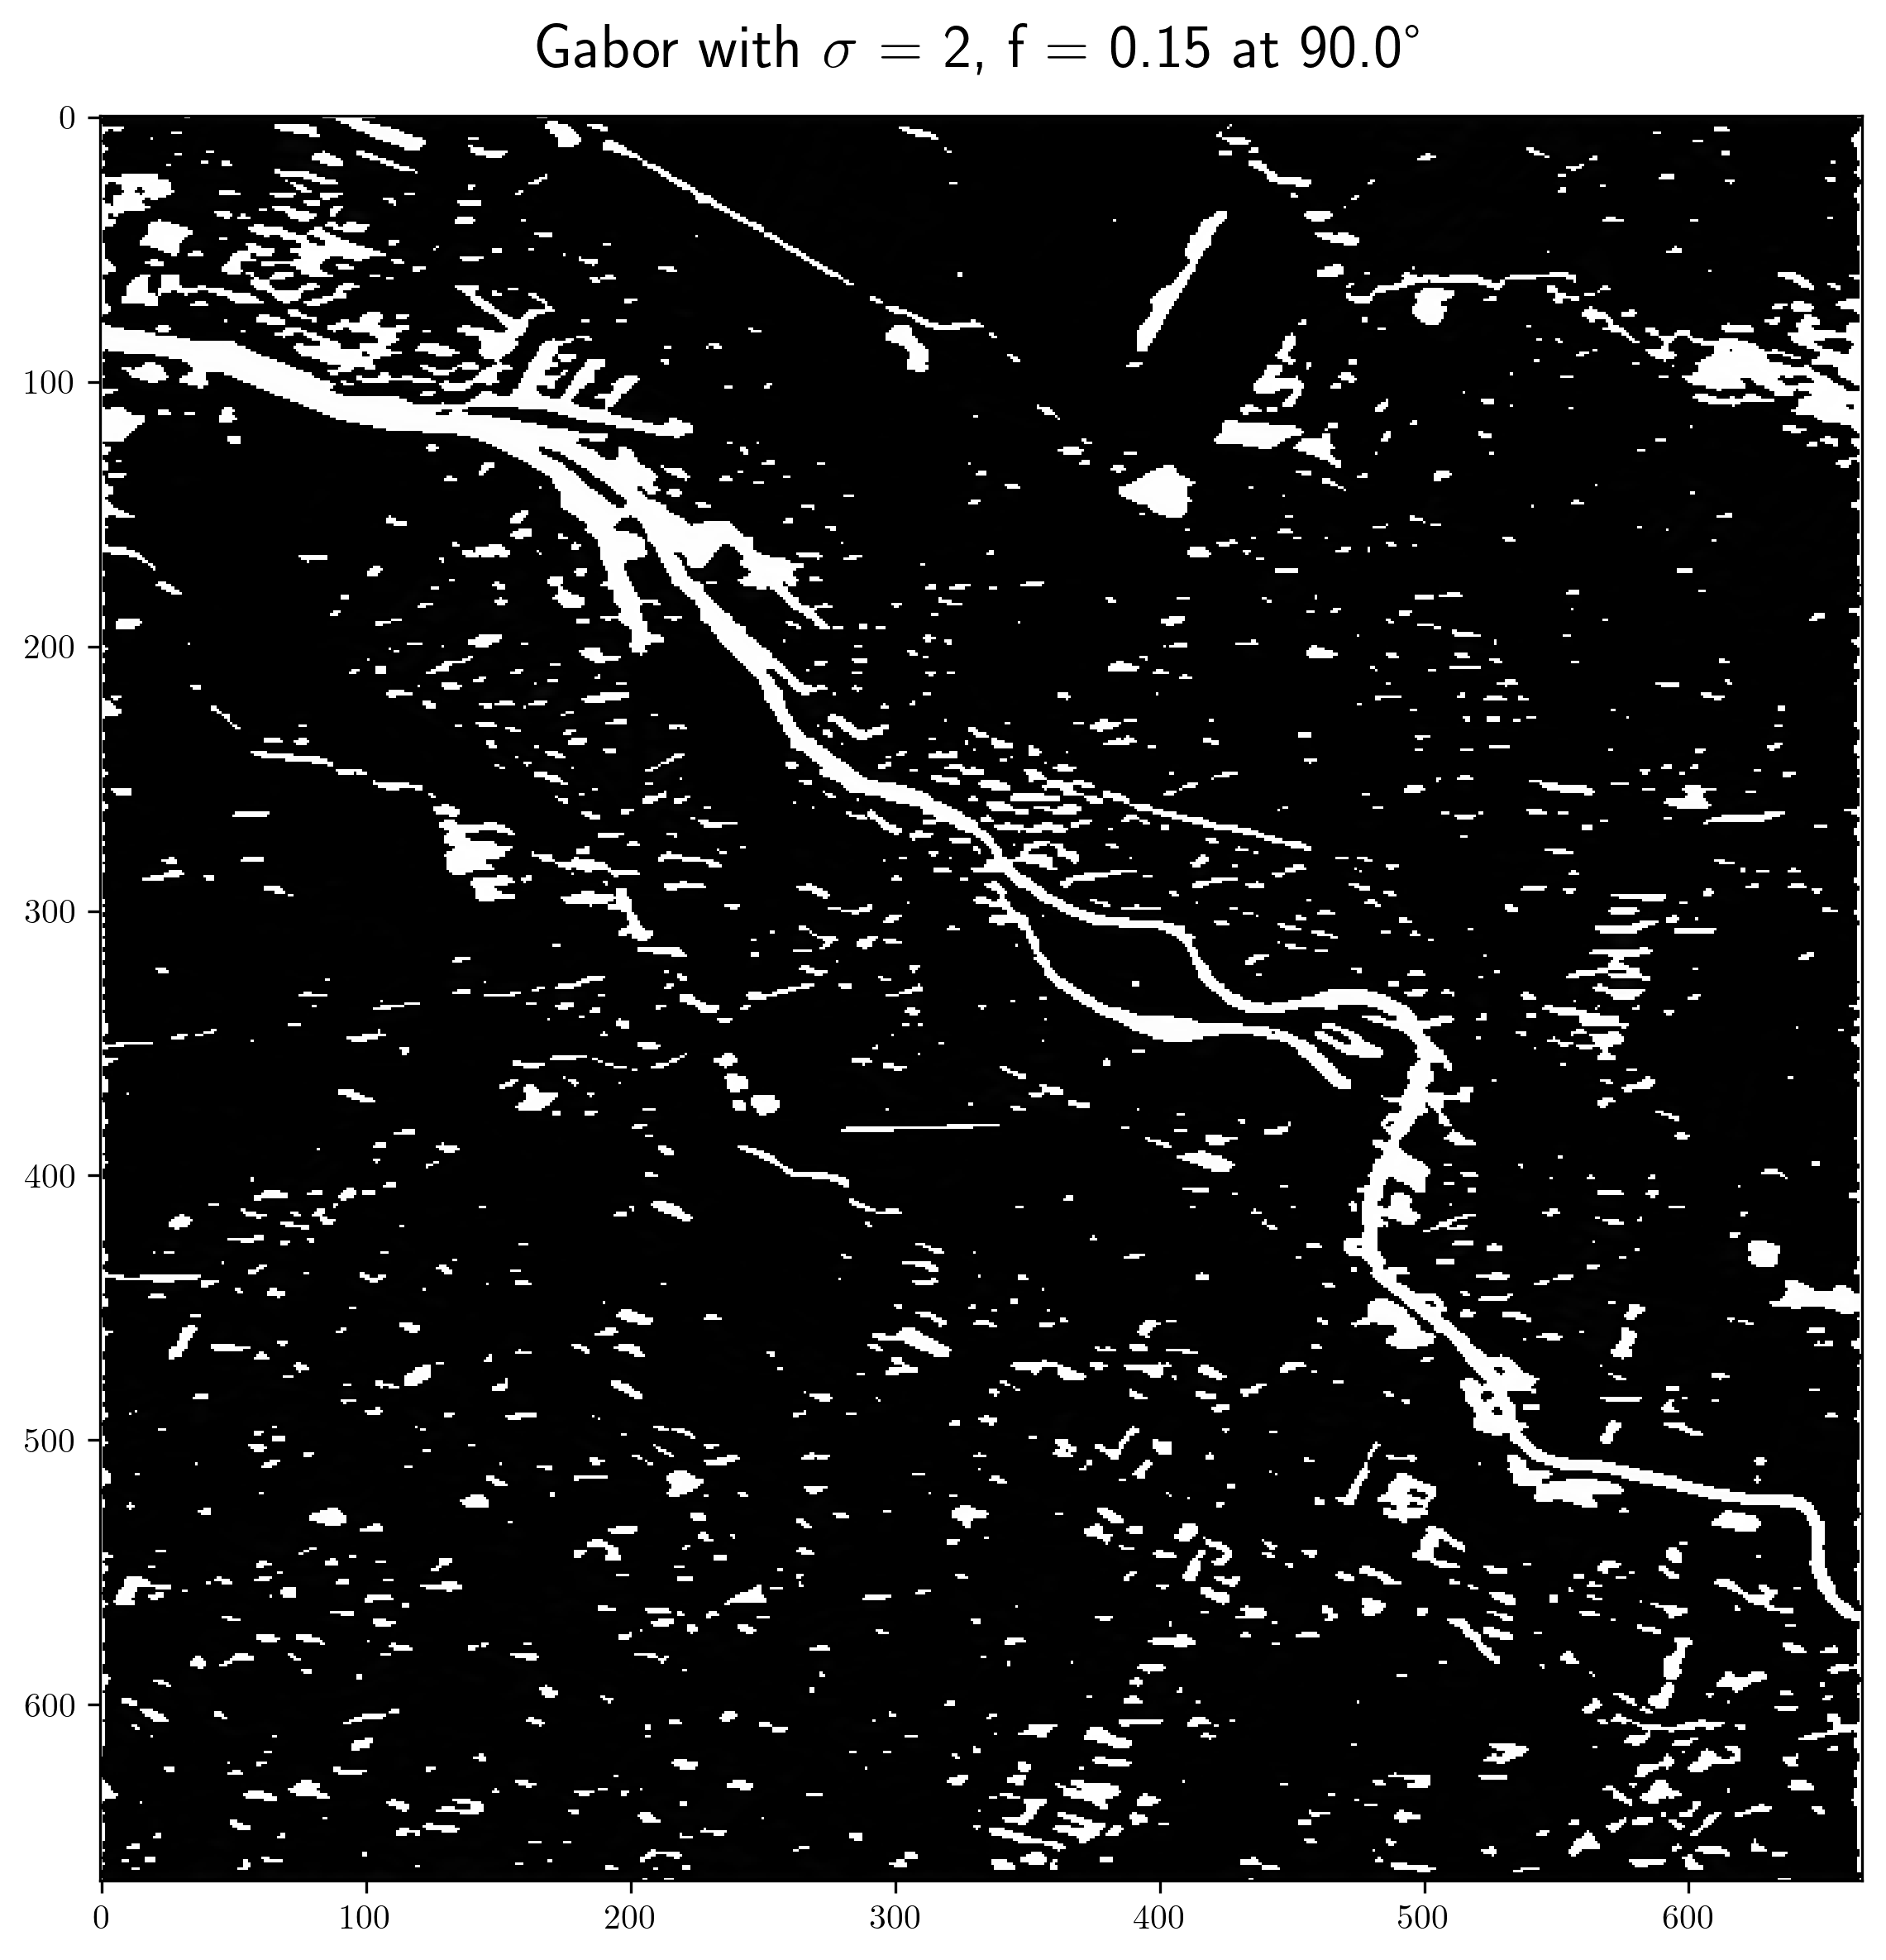
\includegraphics[width=0.85\linewidth]{figures/Features_2_015_90.png}
      \subcaption{Features extracted from an image of the city of Bremen\label{fig:feats}}
    \end{subfigure}
    \vspace{-0.4em}
    \caption{Gabor Filter kernels and convoluted image}
    \end{figure}
  \end{block}

\begin{tikzpicture}
  \node[overlay, remember picture, style=single arrow, fill=UHBRed, shape border rotate=270, minimum width=3cm , minimum height=2.6cm, yshift=2.2cm ,xshift=0.5\colwidth]{};
\end{tikzpicture}

  \begin{block}{Surface Classification}
    Using k-means the surface classes seen in \cref{fig:classes} were determined.
    \vspace{-0.7em}
    \begin{figure}
      \centering
      \begin{subfigure}{0.9\textwidth}
        \centering
        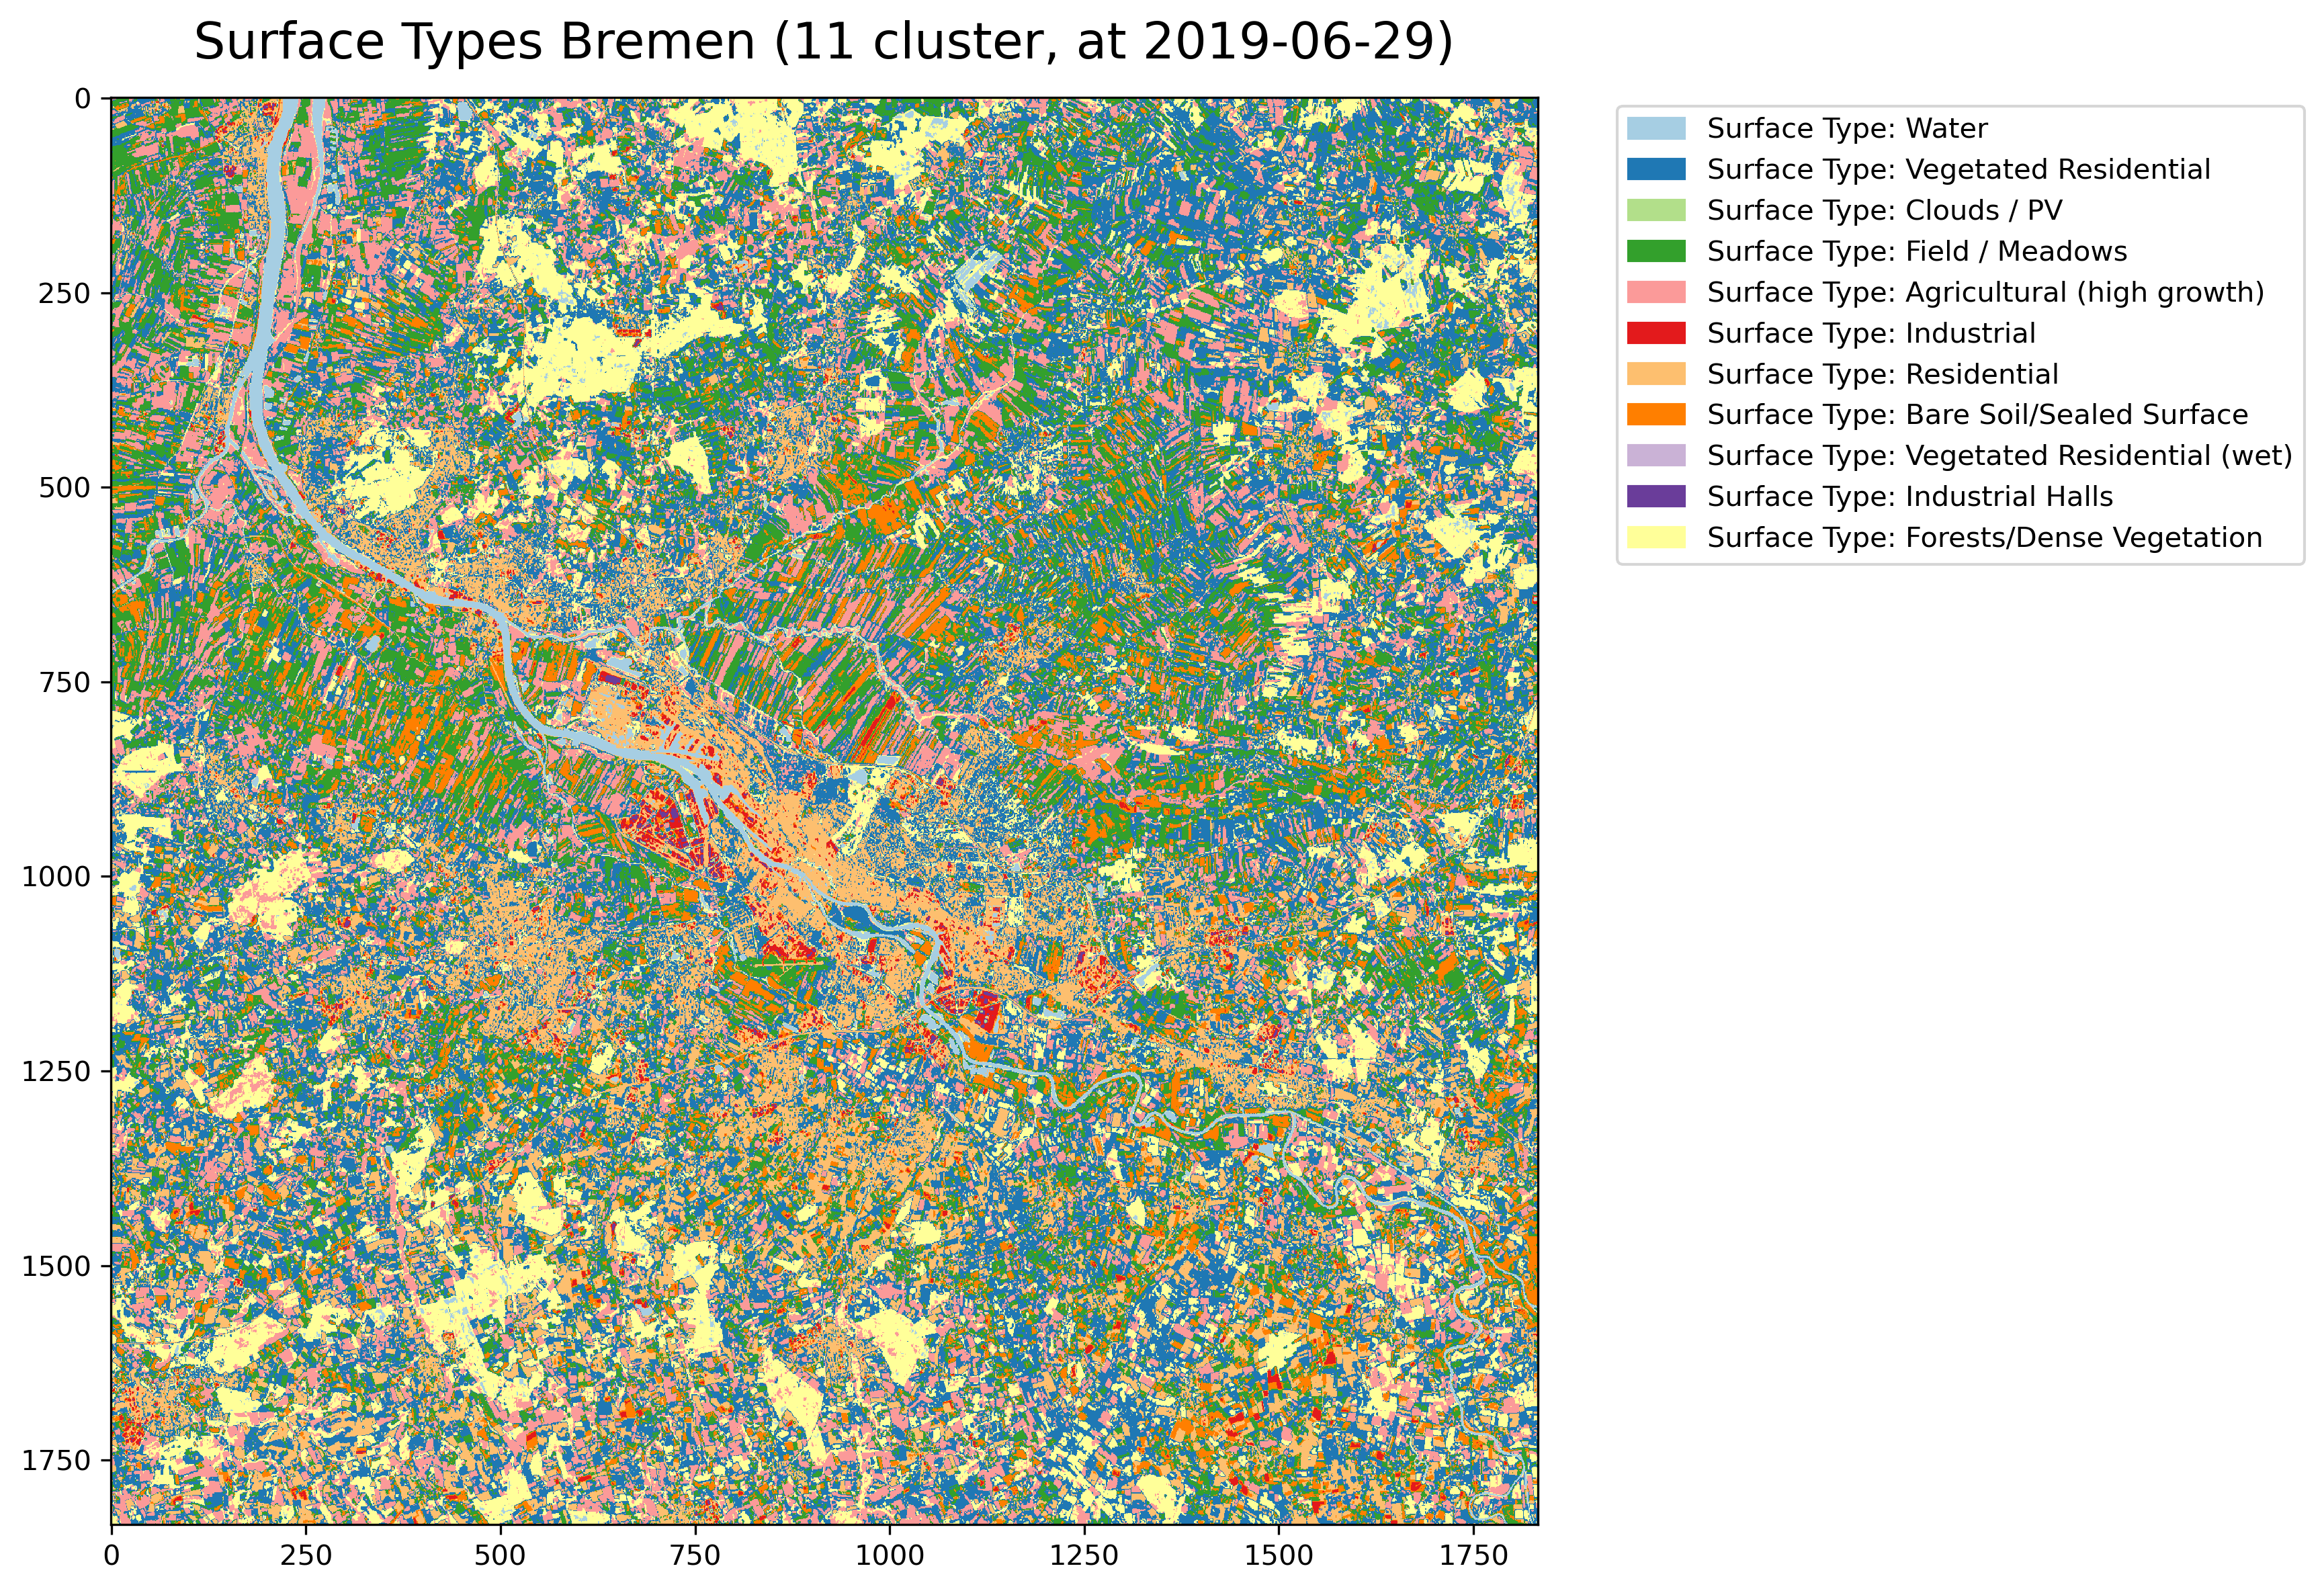
\includegraphics[width=\textwidth]{figures/Classification.png}
        \subcaption{Surface type classification of Bremen and the surrounding area\label{fig:classes}} 
      \end{subfigure}

      \vspace{-0.5em}
      \begin{subfigure}{0.9\textwidth}
        \centering
      \includegraphics[width=0.8\textwidth]{figures/UrbanAreaBremen.png}
      \subcaption{Bremen urban area and the rural buffer zones\label{fig:urban}}
    \end{subfigure}
    \vspace{-2cm}
    \caption{Classification and urban area detection results}
  \end{figure}
  The urban pixels were merged into a continuous urban area with suburban and rural influence zones (\cref{fig:urban}).\\
  \vspace{-2.0em}
  \begin{tikzpicture}
   \node[overlay, style=single arrow, fill=UHBRed, shape border rotate=270, minimum width=3cm, minimum height=2.6cm, yshift=-2.5cm, xshift=0.5\linewidth]{};
  \end{tikzpicture}
  \end{block}
\end{column}

\separatorcolumn%

\begin{column}{\colwidth}

\begin{tikzpicture}
   \node[overlay, style=single arrow, fill=UHBRed, shape border rotate=270, minimum width=3cm, minimum height=2.6cm, yshift=1.8cm ,xshift=0.5\colwidth]{};
\end{tikzpicture}
  
\vspace{0.4em}
  \begin{block}{UHI Detection}
  \begin{figure}
      \centering
      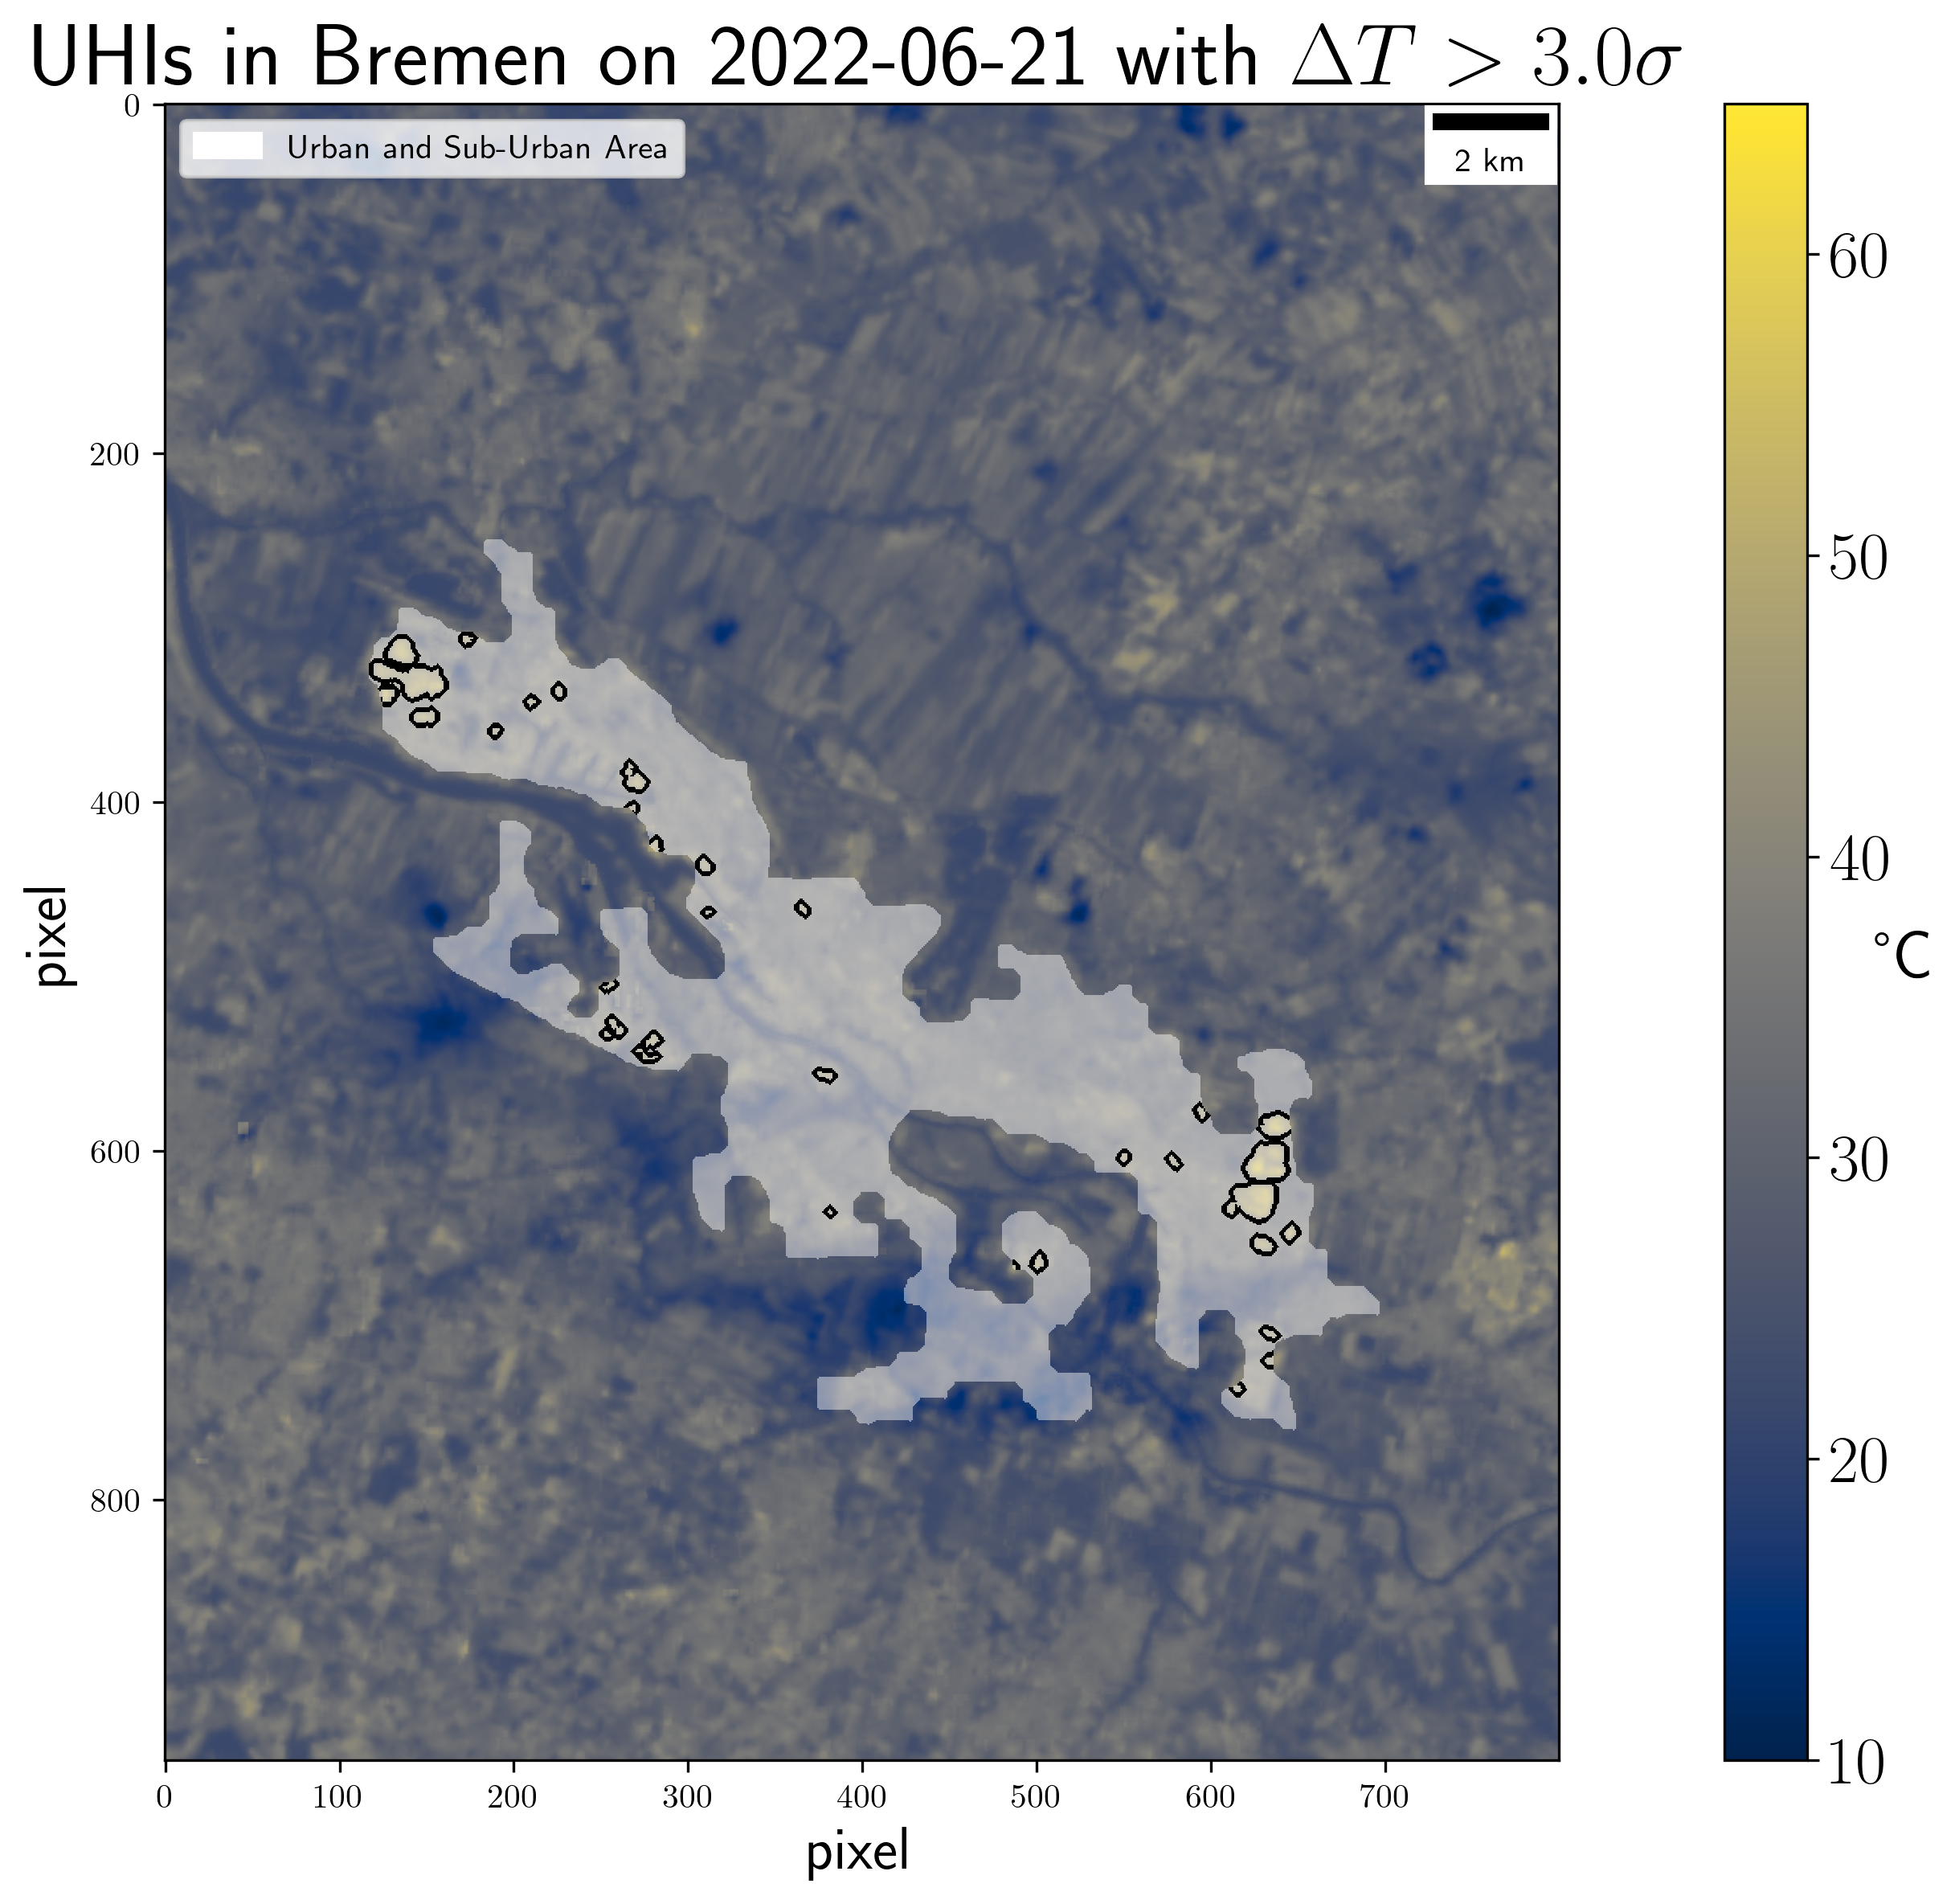
\includegraphics[width=0.9\textwidth]{figures/UHIs_Bremen_2022-06-21_s:3.png}
      \caption{Urban Heat Islands detected in Bremen (more then 3 $\sigma$ above average temp)\label{fig:uhis}}
  \end{figure}
  \end{block}

\vspace{0.4em}
  \begin{tikzpicture}
    \node[overlay, style=single arrow, fill=UHBRed, shape border rotate=270, minimum width=3cm , minimum height=2.6cm, yshift=2.5cm ,xshift=0.5\colwidth]{};
  \end{tikzpicture}

  \begin{block}{Analysis and Results}
    \begin{figure}
        \centering
        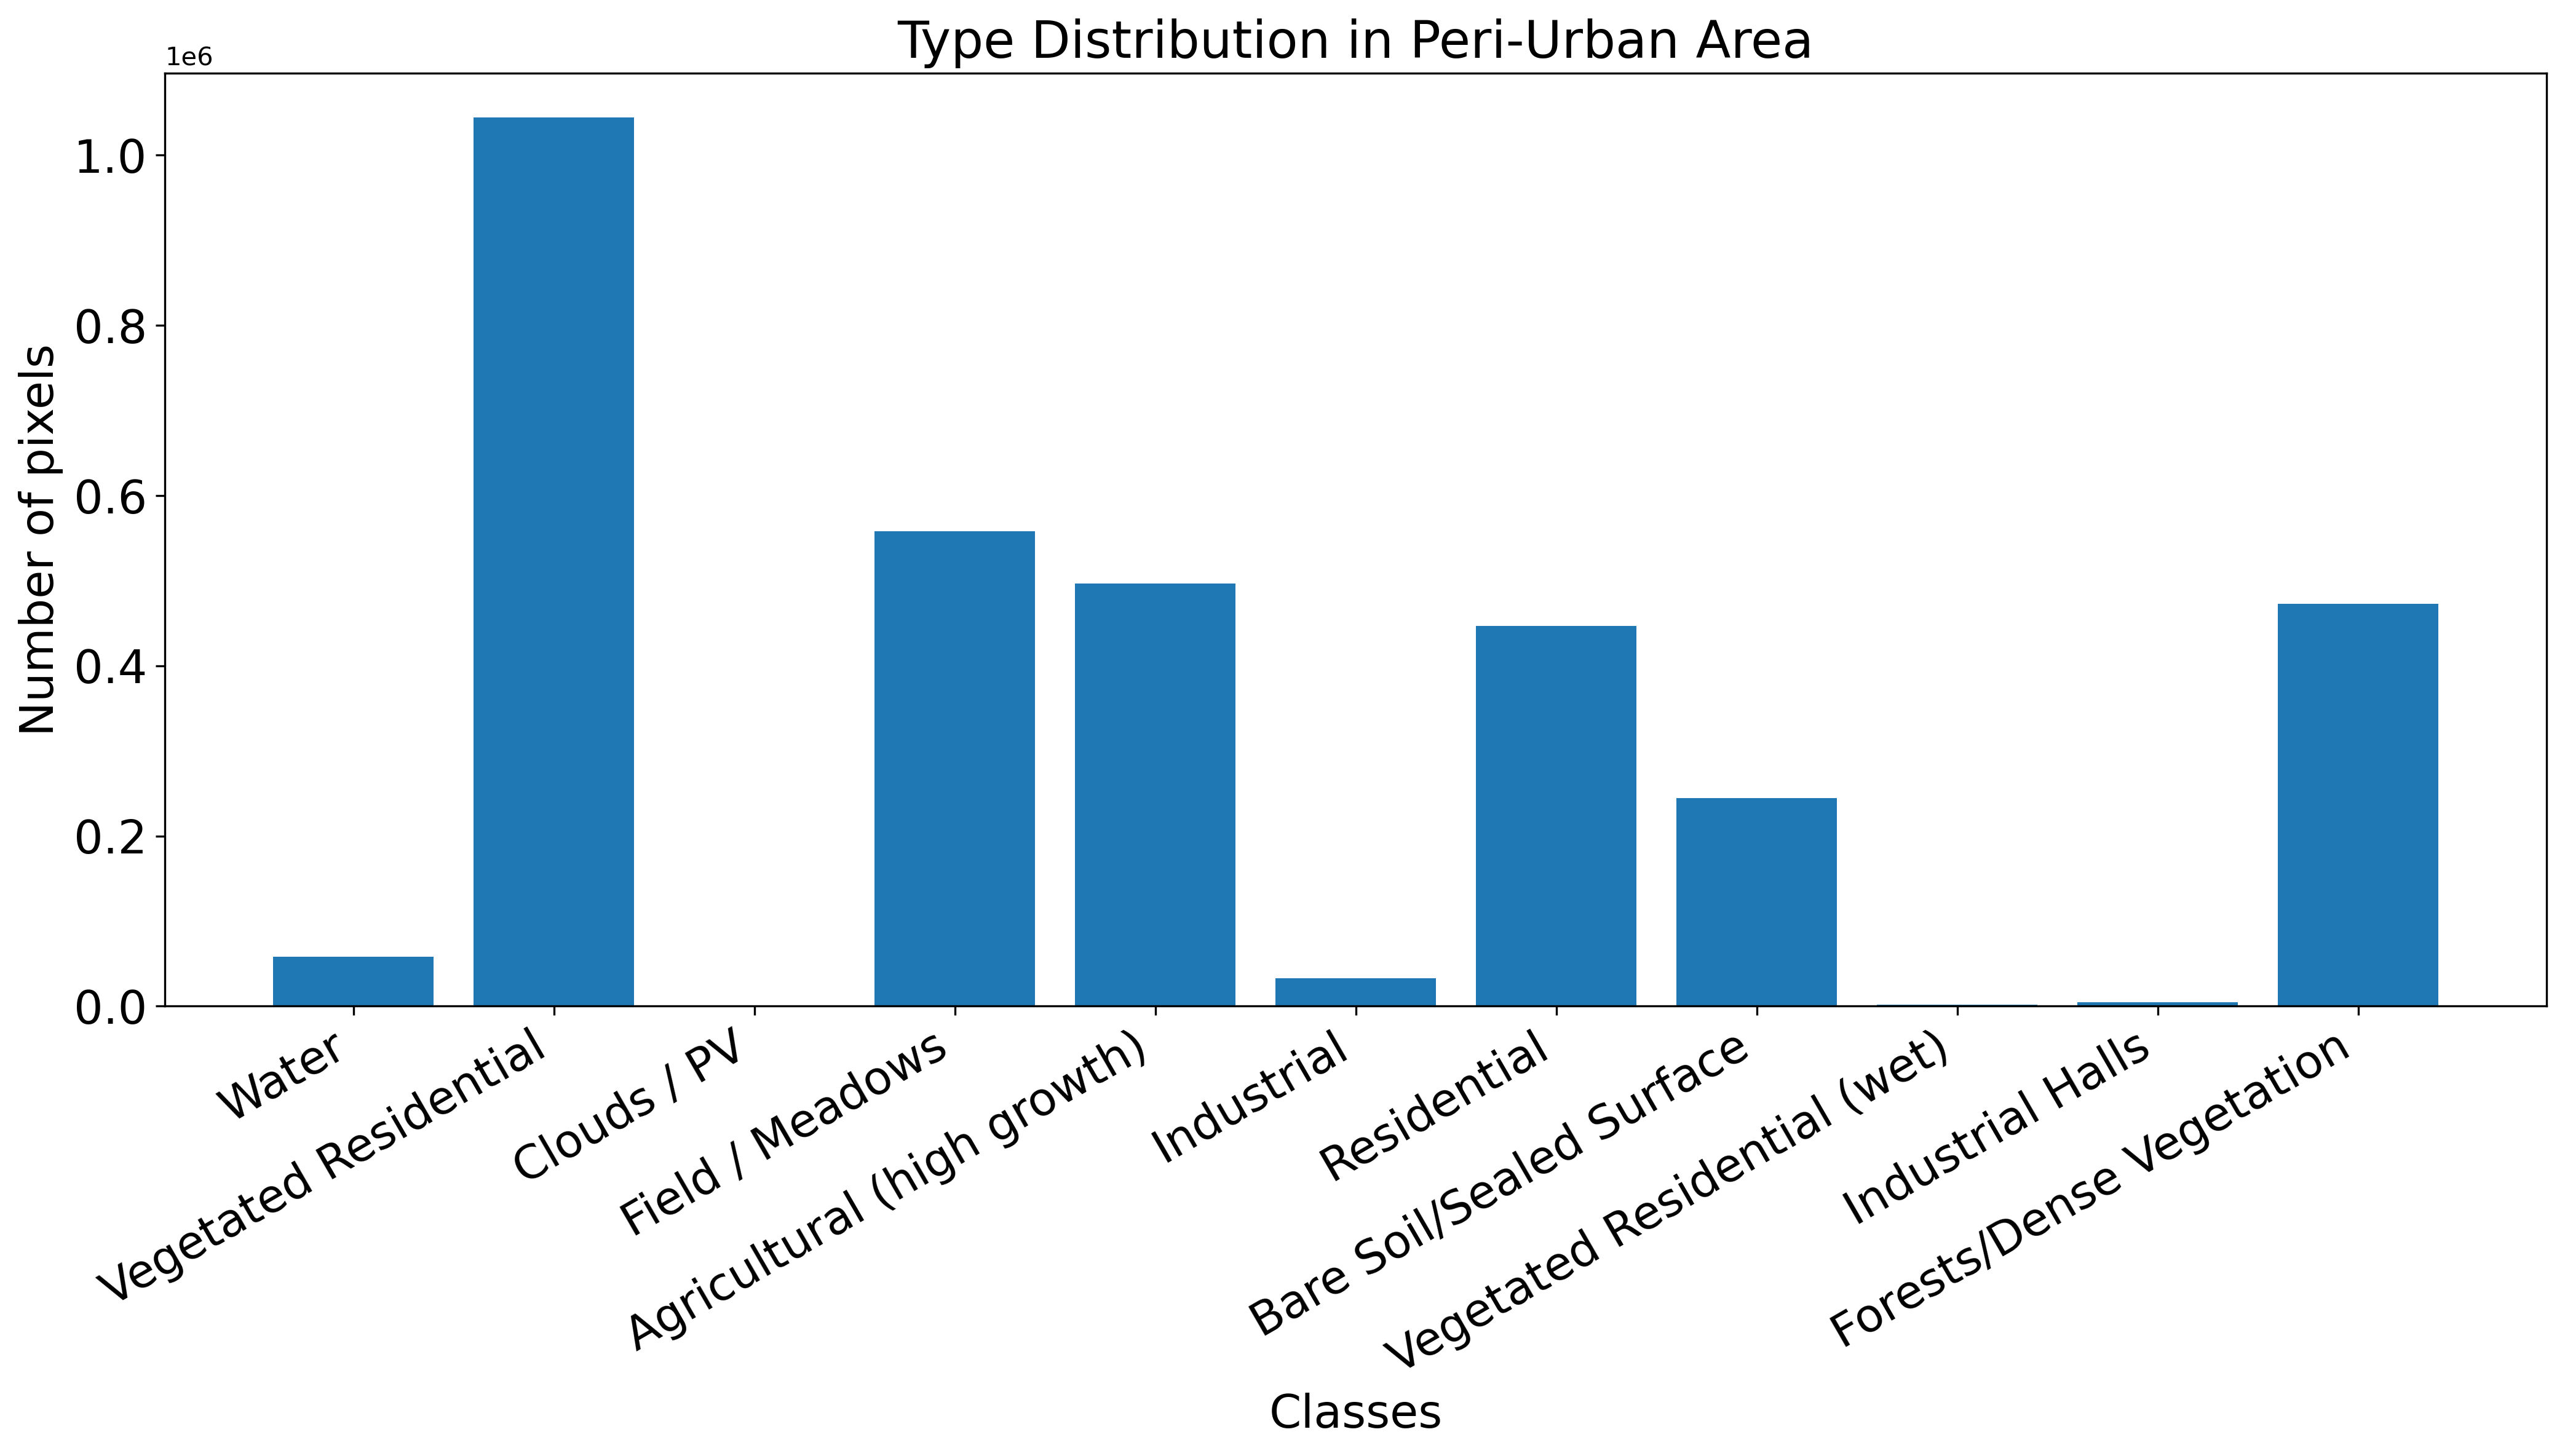
\includegraphics[width=\linewidth]{figures/ClassDistributionPU2019-06-29.png}
        \caption{Statistical analysis of the Bremen surface type distribution within the peri urban area}
    \end{figure}
\vspace{-0.4em}
    \begin{itemize}
      \setlength\itemsep{0.4em}
      \item City area classification works well with the used approach
      \item Detecting surface UHIs works well using Landsat 8 satellite images
      \item Severity depends highly on surface type and weather
      \item An increase in temperatures can be observed in cities at higher latitudes like Bremen
    \end{itemize}
  \end{block}

 % \begin{block}{Next Steps}
 %   \begin{itemize}
 %     \item Time Line
 %   \end{itemize}
 % \end{block}
  \vspace{-1.5cm}
  \begin{alertblock}{Summery}
    \begin{itemize}
      \setlength\itemsep{0.5em}
      \item Remote sensing data can help with detection and monitoring of UHIs
      \item UHI increase in size and merge to larger scale structures with increased mean temperature
      \item Maximum temperature of UHI is not increasing as strongly 
      \item More studies need to be conducted, using multiple datasets for statistical analysis
    \end{itemize}
  \end{alertblock}

  \vspace{-1.5cm}
  \begin{block}{Reference}
    Read the Thesis here:\\
      \href{https://github.com/paradx/mscthesis/releases/download/printed/thesis\_singleSided.pdf?raw=true}{https://github.com/paradx/mscthesis/releases/download/printed/thesis\_singleSided.pdf?raw=true}
%    \nocite{*}
%    \footnotesize{\printbibliography}
  \end{block}

\end{column}

\separatorcolumn%
\end{columns}
\end{frame}

\end{document}
% EOF
